\documentclass[11pt,handout]{beamer}
\usepackage{pgfpages}

\usepackage[utf8]{inputenc}
\usepackage[T1]{fontenc}
\usepackage{lmodern}
\usepackage{graphicx}
\usepackage{rail}
\usepackage[french]{babel}
\usepackage{listings} 
\usepackage{xcolor}
\usetheme{Goettingen}
\usecolortheme{sidebartab}
\setbeamertemplate{itemize item}[ball]
\setbeameroption{show notes}
%\setbeameroption{hide notes}

\lstdefinelanguage{Stibbons}{
  morekeywords={
    new,agent,for,repeat,while,fd,forward,lt,turn-left,rt,turn-right,pd,pen-down,pu,pen-up,
    if,else,true,false,and,or,xor,not,function,null,null\_t,number\_t,boolean\_t,string\_t,
    color\_t,table\_t,turtle\_t,zone\_t,world\_t,send,recv,die
  },
  sensitive=false,
  morecomment=[s]{/*}{*/},
  morecomment=[l]{//},
  morestring=[b]',
  morestring=[b]",
}

\lstset{
  breaklines=true,
  captionpos=b,
  showstringspaces=true,
  tabsize=2,
  language=C++,
  frame=simple,
  float,
  floatplacement=H
}

\railalias{dot}{.}
\railterm{dot}

\title{Stibbons}
\author{Bassoumi Julia \\ Galinier Florian \\ Plazas Adrien \\ Simon Clément}
\date{\today}

\begin{document}

\begin{frame}
\titlepage
\end{frame}

\begin{frame}
\tableofcontents
\end{frame}

\section{Introduction}
\begin{frame}
\begin{itemize}
	\item Dérivé de Logo
		
\includegraphics[scale=0.4]{doc/Presentation/image/logo.pdf}
	\item Inspiré de NetLogo et de StarLogo
		
\includegraphics[scale=0.3]{doc/Presentation/image/netlogo.pdf}
		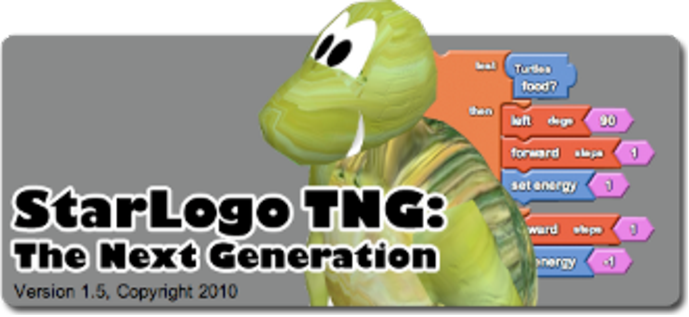
\includegraphics[scale=0.4]{doc/Presentation/image/starlogo.pdf}
\end{itemize}
\end{frame}

\begin{frame}
\frametitle{Le Projet Stibbons}
\begin{itemize}
	\item Un langage de programmation multi-agents
	\item Un interprète de ce langage
	\item Une application graphique
\end{itemize}
\end{frame}


\section{Le Stibbons}
\begin{frame}[fragile]
	\small
	\begin{lstlisting}[language=Stibbons]
new agent {
  a = 10
  fd a + 2
}

agent turtle (a) {
  teleport(random(0,world.max_x),
           random(0,world.max_y),
           rand())
  pd
  function f (w, c) {
    fd w
    rt 360 / c
  }
  repeat a {
    f(10, a)
  }
}

5 new turtle (4)
	\end{lstlisting}
\end{frame}

 
\section{Interprète}
\begin{frame}
La partie interprete est constitué de 3 analyseurs~:
\begin{enumerate}
\item analyseur lexical (Flex)~;
\item analyseur syntaxique (Bison)~;
\item analyseur sémantique (C++).
\end{enumerate}
\end{frame}

\subsection{Analyse lexical}
\begin{frame}
	\frametitle{Analyseur lexical}
	\begin{description}
		\item [Objectif] Génération de jetons
		\item [Méthode] Détection de lexèmes par des expressions régulières
		\item [Outil] GNU Flex (Lex)
	\end{description}
\end{frame}

\begin{frame}[fragile]
	\begin{rail}
		NUMBER : (('0-9' + ) \\ ( (dot ( '0-9' * ) ) ?))
		| dot ( '0-9' + ) ;
	\end{rail}
\end{frame}

\begin{frame}[fragile]
	Code~:
	\begin{lstlisting}[language=Stibbons]
new agent {
  a = 10
  fd a + 2
}
	\end{lstlisting}
	Jetons~:
	\begin{lstlisting}[breaklines]
<NEW> <AGT> <{> <\n> 
<ID,"a"> <=> <NUMBER,10> <\n>
<FD> <ID,"a"> <+> <NUMBER,2> <\n>
<}>
	\end{lstlisting}
\end{frame}


\subsection{Analyse syntaxique}
\begin{frame}
	\begin{itemize}
	\item Objectif double~: 
		\begin{itemize}
		\item Vérifier la validité du programme écrit~;
		\item Générer un arbre abstrait analysable par l'analyseur sémantique.
		\end{itemize}
	\item Langage utilisé~: GNU Bison.
	\end{itemize}
\end{frame}

\begin{frame}
L'exemple précédent génère l'abre abstrait suivant~:
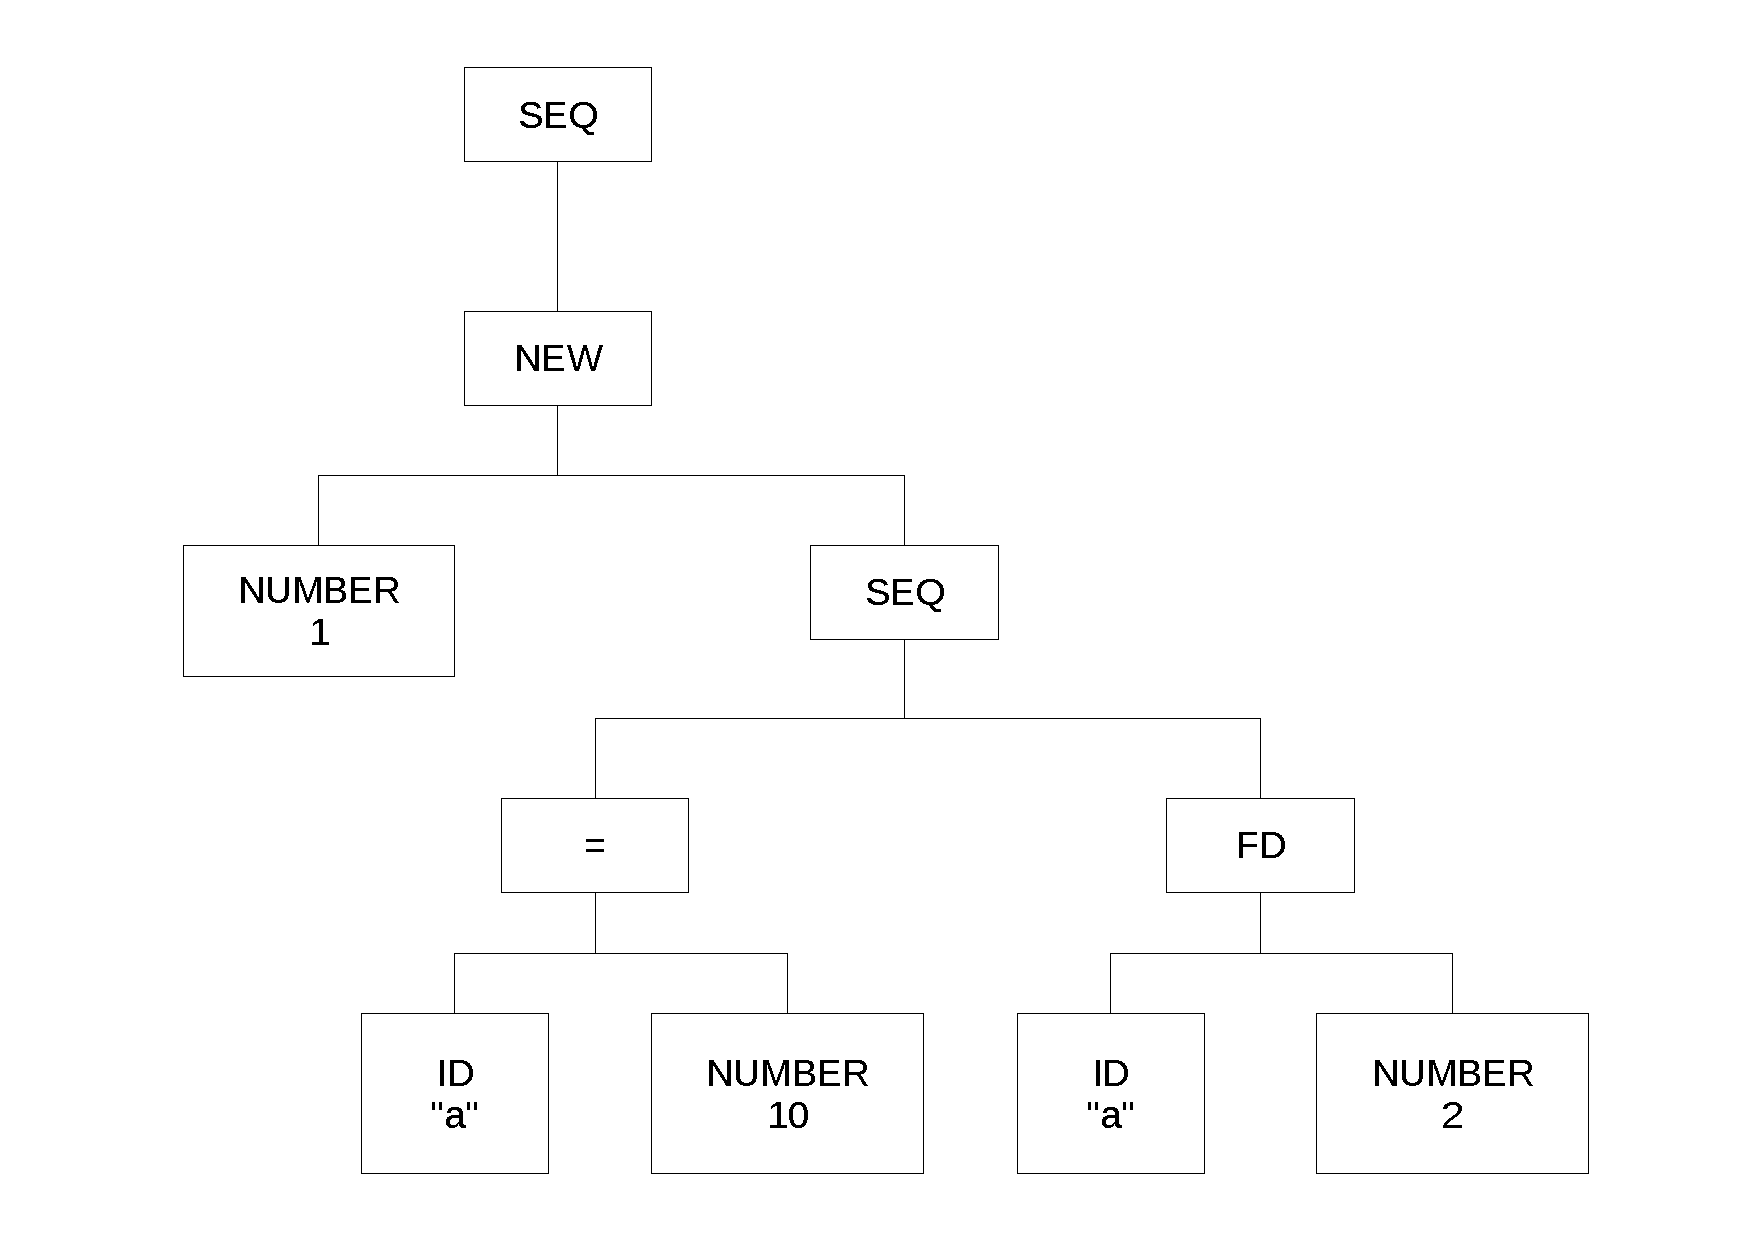
\includegraphics[scale=0.3]{doc/Presentation/img/arbre.pdf}
\end{frame}



\subsection{Analyse sémantique}
\input{doc/Presentation/sémantique.tex}


\section{Modèle}
\subsection{Les classes agents}
\begin{frame}
\frametitle{Modèle}
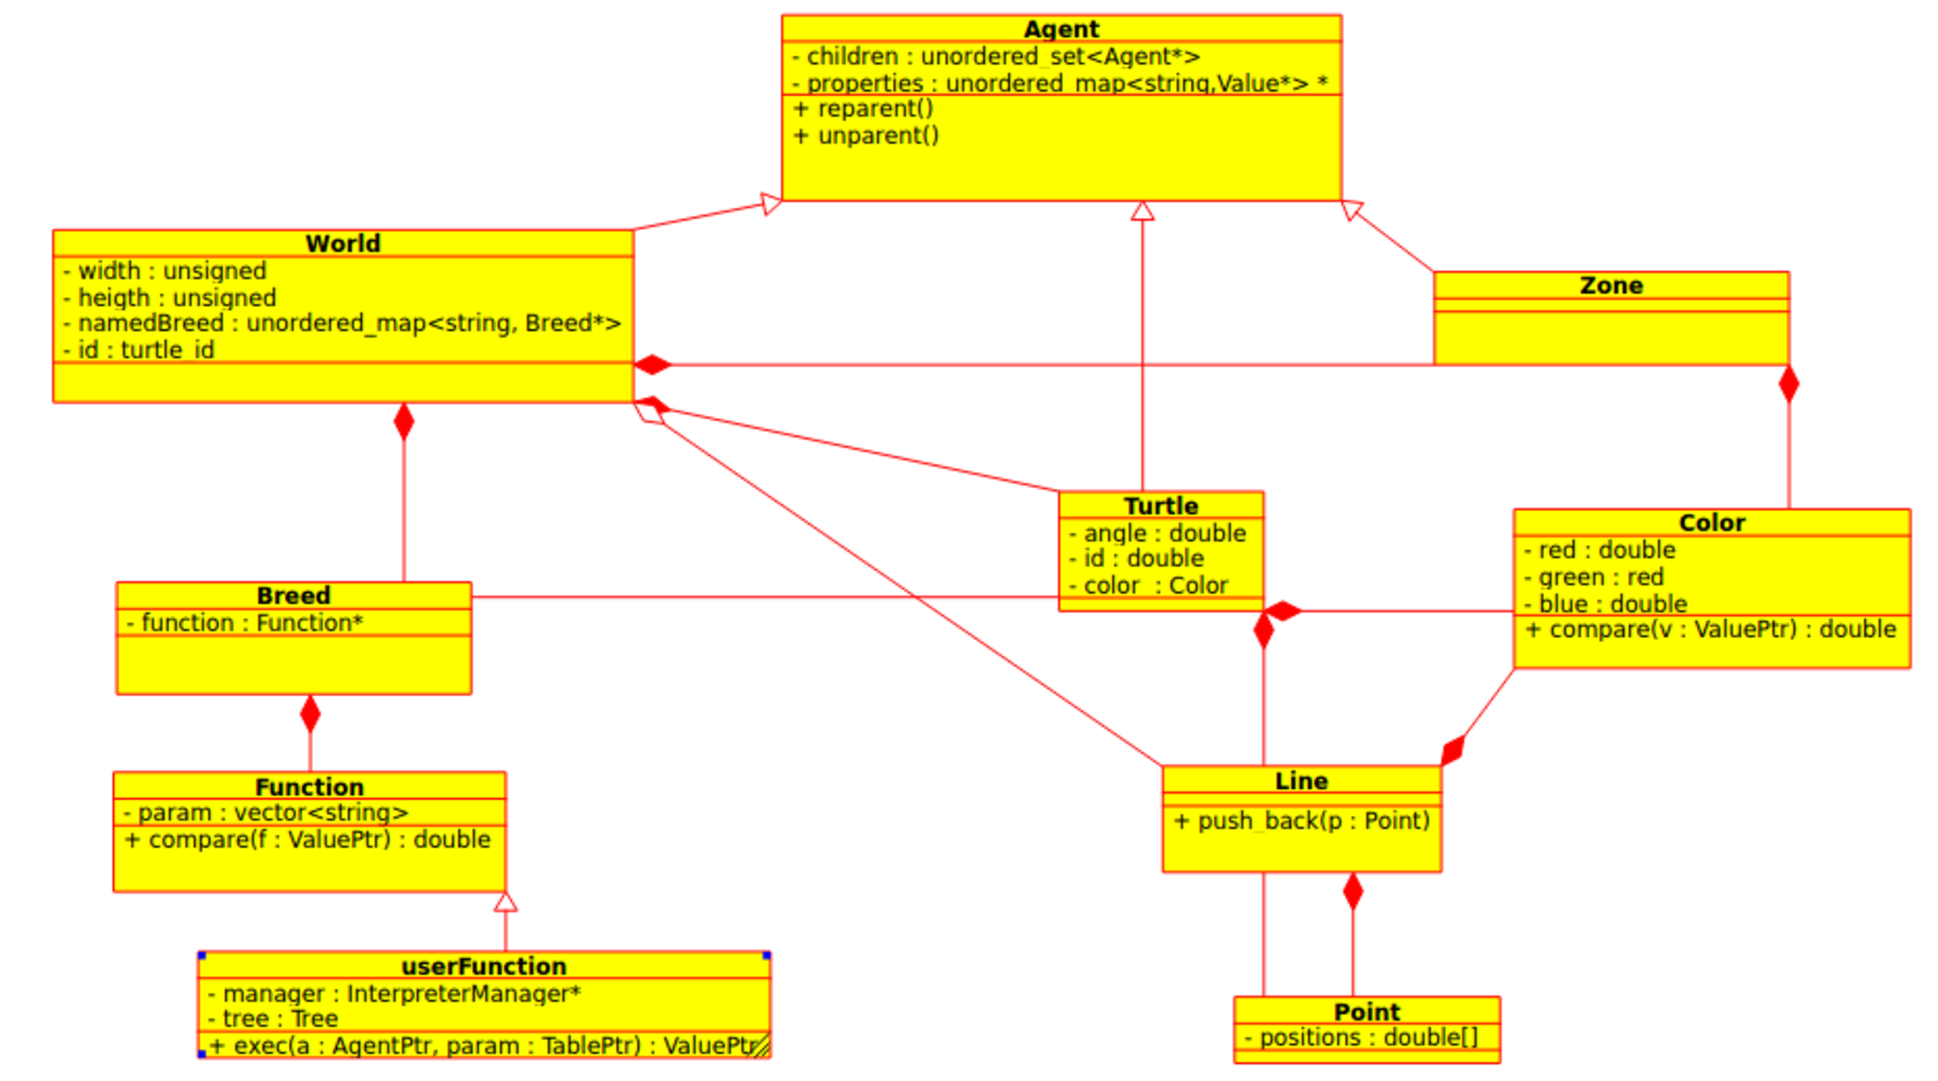
\includegraphics[scale=0.31]{doc/Presentation/image/agents.pdf}
\end{frame}

\note{diagramme=modèle à l'état final.\\
Sprint 1 : turtle point, line, world. Détail...\\
Sprint 2 : classes agent(regroupe comportement) et breed(nommée ou pas), ajout des fonctions, qui stocke un arbre abstrait, contenant le code de la fonction déjà analysé.; Détail....\\
Sprint 3 : les communications : zones propriétés et tortues send, recv...\\
 			export : méthode dans chaque agent\\
 			ajout user function
}

\subsection{Les types}
\begin{frame}
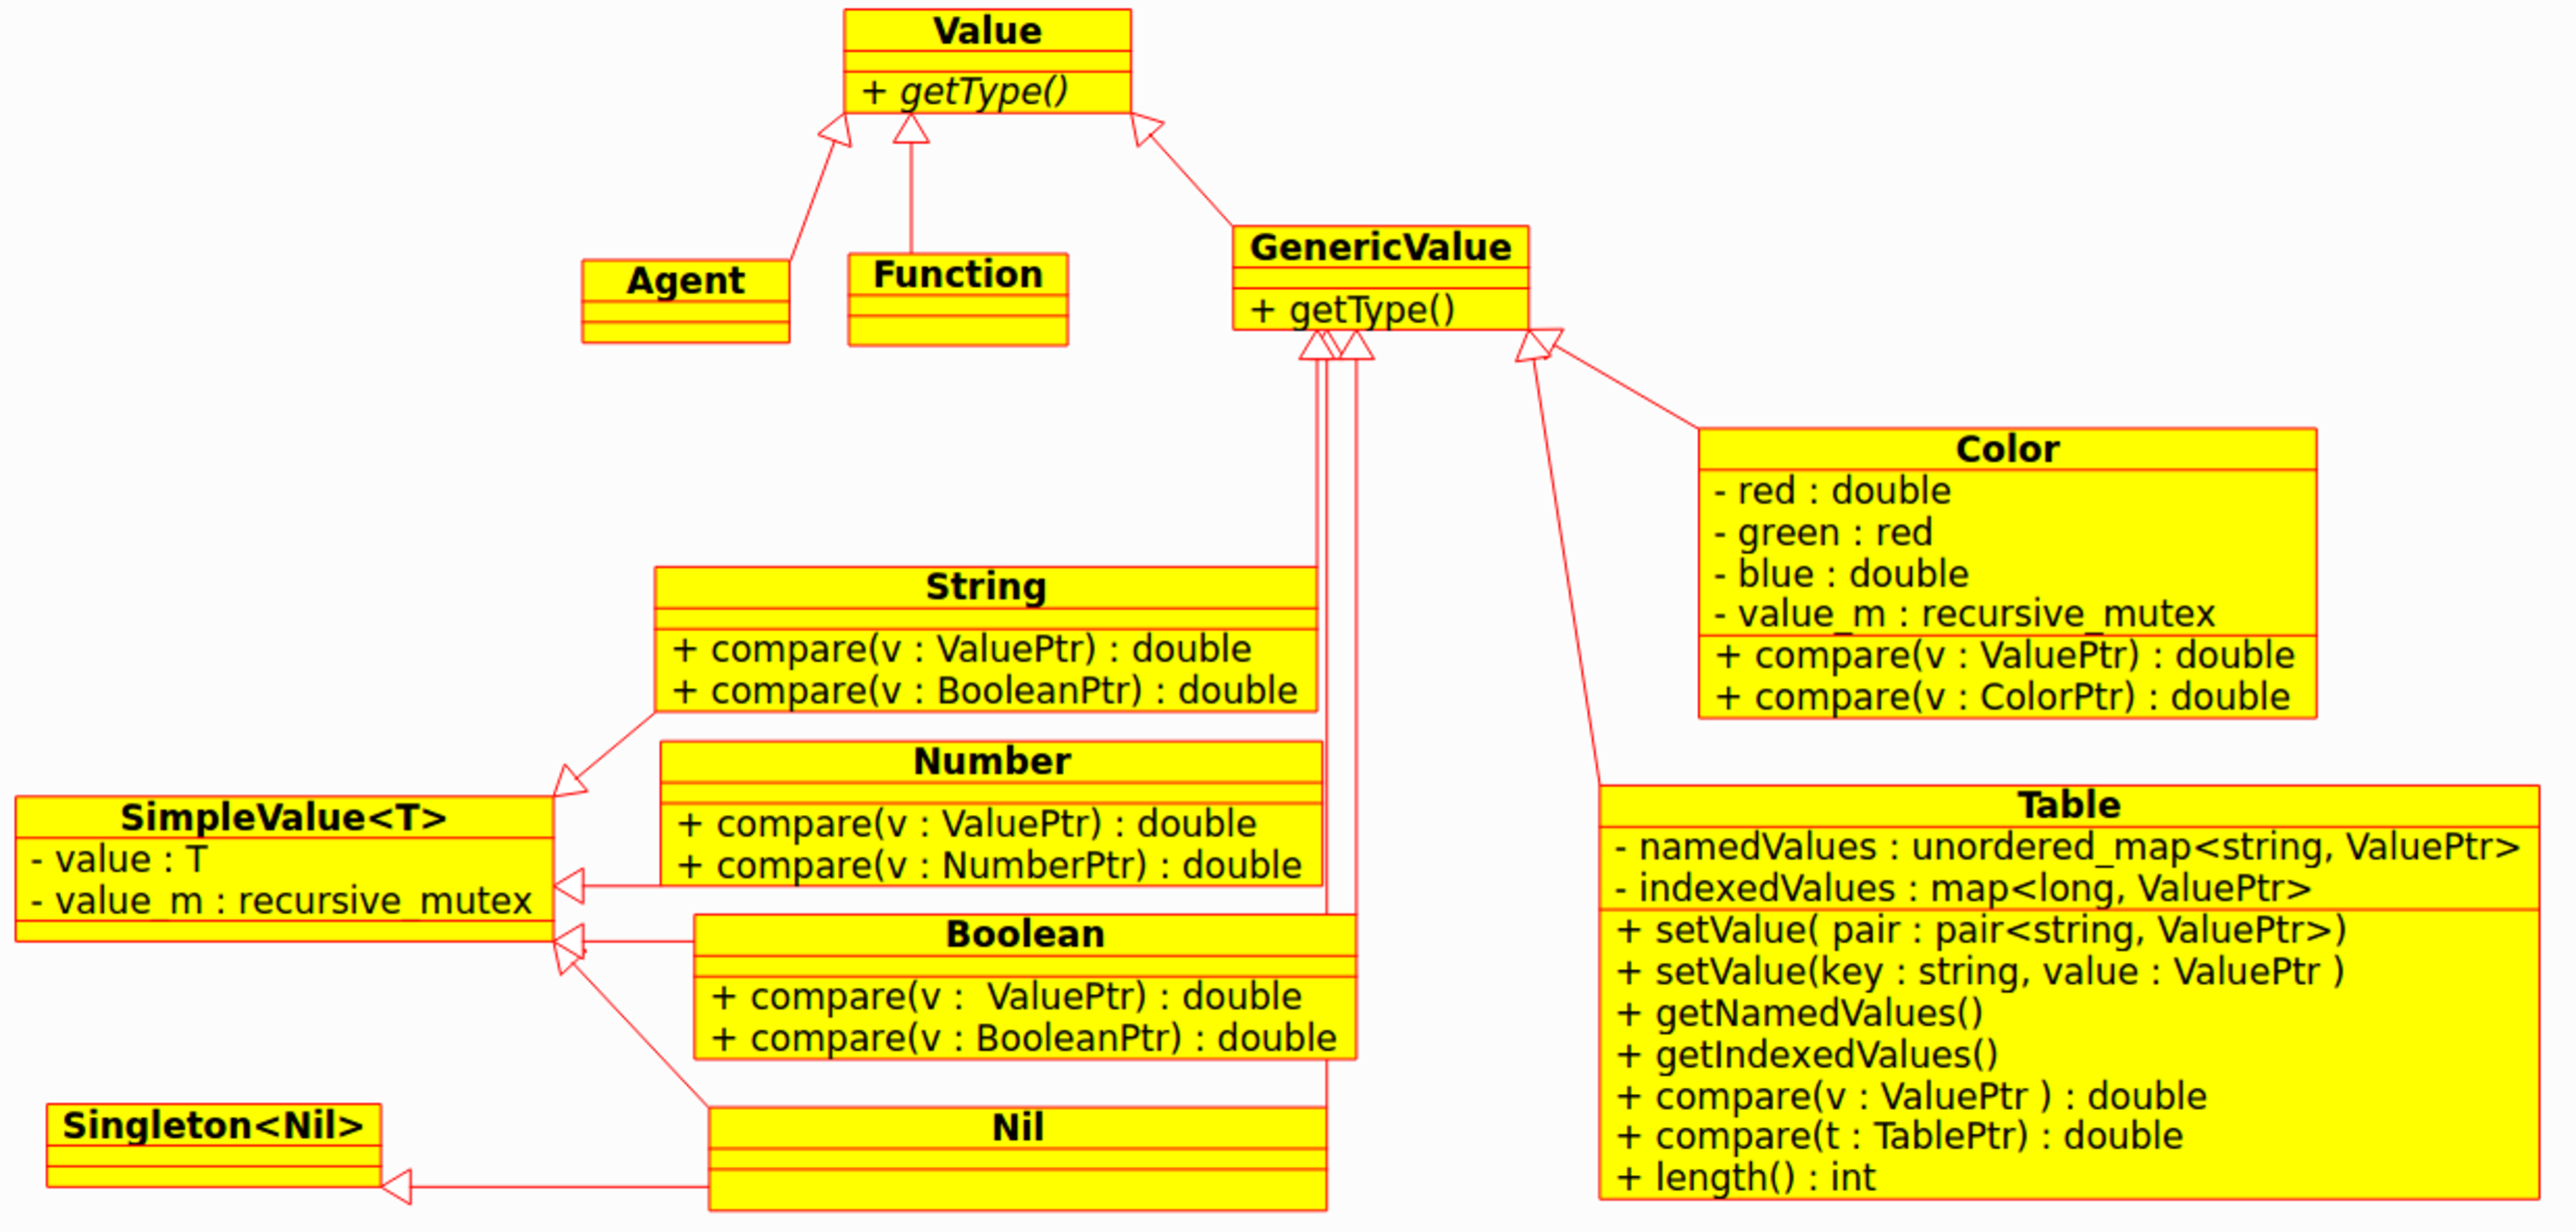
\includegraphics[scale=0.27]{doc/Presentation/image/types.pdf}
\end{frame}
\note{1er sprint : color nil et value\\
2eme : compléxifié avec simple value pour les mutexs\\
4eme : table et mutex recursifs
}


\section{Organisation}
\begin{frame}
\frametitle{Organisation}
Méthode agile : Scrum
\begin{itemize}
\item Méthode itérative
\item Temps divisé en sprints
\item Backlog
\end{itemize}
\end{frame}


\begin{frame}
\frametitle{Backlog}
{\tiny
\begin{longtable}[c]{|c|p{1cm}|c|p{1.7cm}|*{4}{c|}}
\hline
\bf id & \bf Scénario utilisateur & \bf Priorité & \bf Tests & \bf Estimation & \bf Sprint & \bf Statut & \bf Temps réel \\
\hline
\endfirsthead
\hline
\bf id & \bf Scénario utilisateur & \bf Priorité & \bf Tests & \bf Estimation & \bf Sprint & \bf Statut & \bf Temps réel \\
\hline
\endhead
1 & L'utilisateur écrit du code dans un éditeur & 200 & L'utilisateur écrit du code dans un éditeur intégré & & & & \\
\hline
2 & L'utilisateur importe du code dans le logiciel & 1100 & Importer du code Stibbons depuis un fichier, vérifier que le code obtenu est bien identique à celui du fichier. & 4h & 1 & Fini & 1h \\
\hline
3 & L'utilisateur visualise les rapports d'erreurs du code & 400 & Exécuter pd 50 et constater une erreur. & 8h & 4 & Fini & 8h \\
\hline
4 & L'utilisateur visualise l'évolution du modèle & 1400 & Vérifier que l'interprétation d'instructions données fait bien évoluer comme prévu la tortue dans son environnement. & 24h & 1 & Fini & 70h \\
\hline
\end{longtable}}
\end{frame}

\begin{frame}
\frametitle{Outils}
\begin{center}
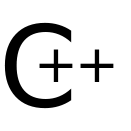
\includegraphics[height=50px]{doc/Presentation/image/cpp.png}

\includegraphics[height=50px]{doc/Presentation/image/qt.jpg}

\includegraphics[height=50px]{doc/Presentation/image/gnu.png}\\

\includegraphics[width=50px]{doc/Presentation/image/cppUnit.pdf}

\includegraphics[width=50px]{doc/Presentation/image/jsonspirit.pdf}
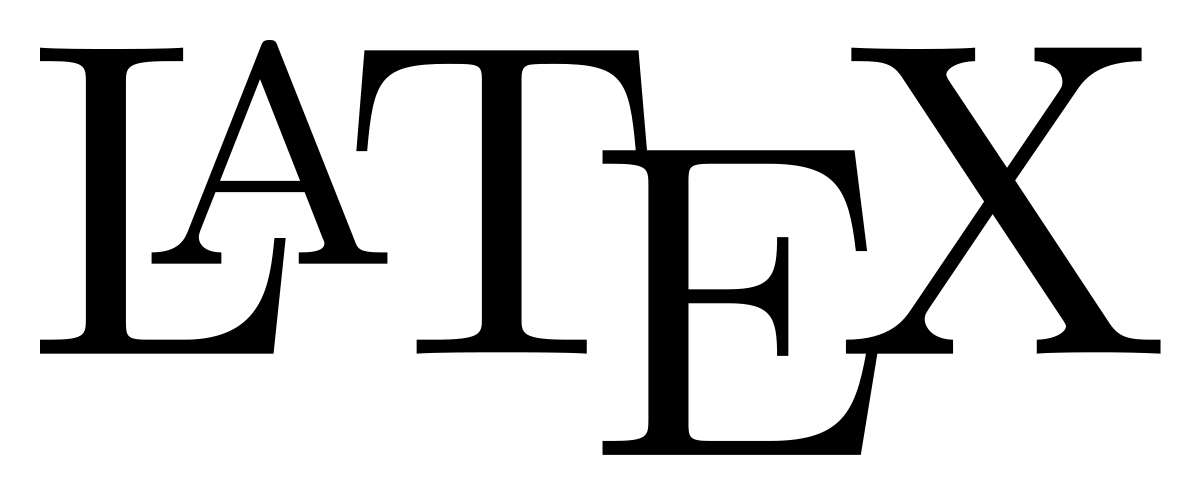
\includegraphics[width=50px]{doc/Presentation/image/latex.png}\\

\includegraphics[height=50px]{doc/Presentation/image/git.pdf}

\includegraphics[height=50px]{doc/Presentation/image/gitg.png}

\includegraphics[height=50px]{doc/Presentation/image/gitlab.pdf}
\end{center}
\end{frame}


\section{Application}
\subsection{Application graphique}

\begin{frame}
\frametitle{Application graphique v0.1}
\begin{center}
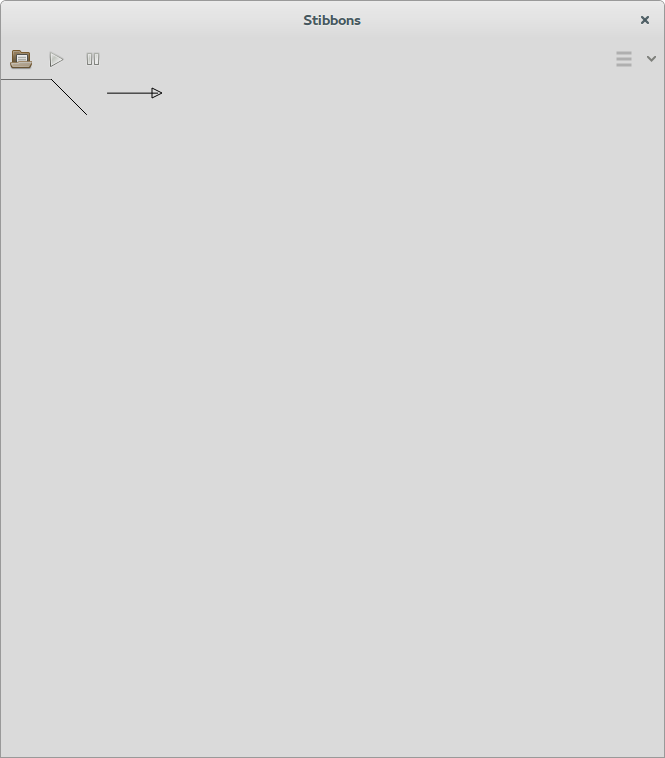
\includegraphics[scale=0.16]{doc/Presentation/screenshot/stibbons-0-1-2.png}
\end{center}

\begin{itemize}
	\item Une tortue par défaut
	\item Tortue = triangle noir creux
	\item La tortue peut tracer des lignes
	\item Origine dans le coin supérieur gauche
	\item Impossible d'ouvrir plusieurs programmes
\end{itemize}
\end{frame}

\begin{frame}
\frametitle{Application graphique v0.2}
\begin{center}
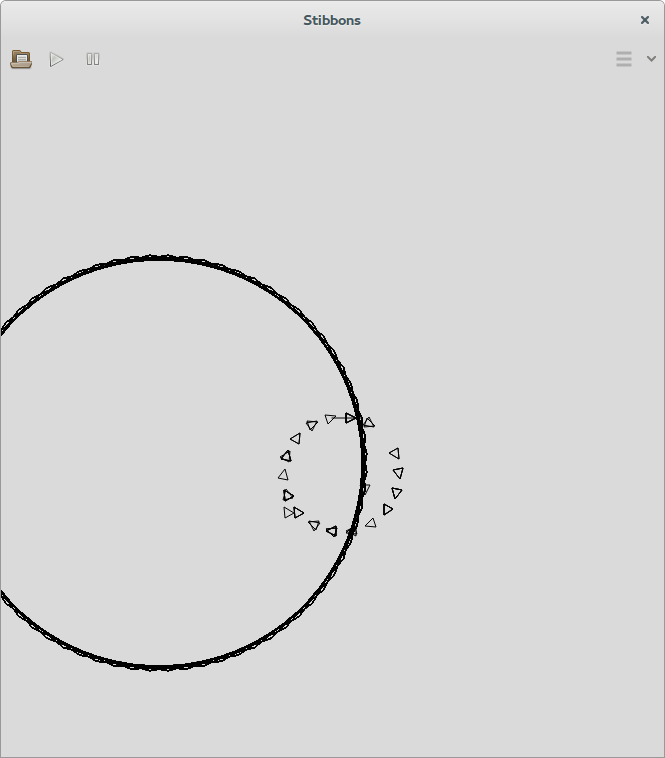
\includegraphics[scale=0.16]{doc/Presentation/screenshot/stibbons-0-2-2.png}
\end{center}

\begin{itemize}
	\item Possibilité de créer d'autres tortues
	\item Origine centrée
\end{itemize}
\end{frame}

\begin{frame}
\frametitle{Application graphique v0.3}
\begin{center}
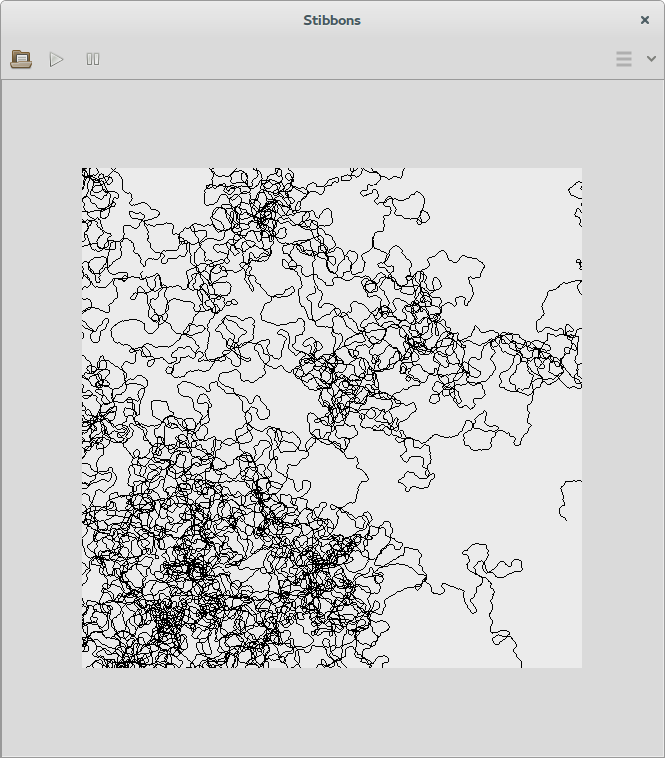
\includegraphics[scale=0.16]{doc/Presentation/screenshot/stibbons-0-3-2.png}
~~~~~~~~
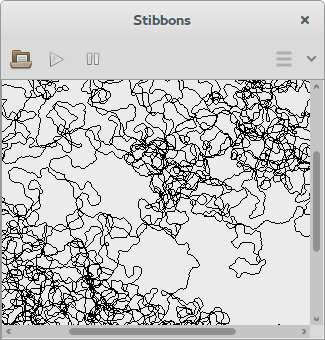
\includegraphics[scale=0.16]{doc/Presentation/screenshot/stibbons-0-3-3.png}
\end{center}

\begin{itemize}
	\item Monde borné, centré
	\item Tortues colorées, dessinées pleines
	\item Lignes colorées
	\item Zones visibles et colorées
	\item Performances de dessin améliorées
\end{itemize}
\end{frame}

\begin{frame}
\frametitle{Application graphique v0.4}
\begin{center}
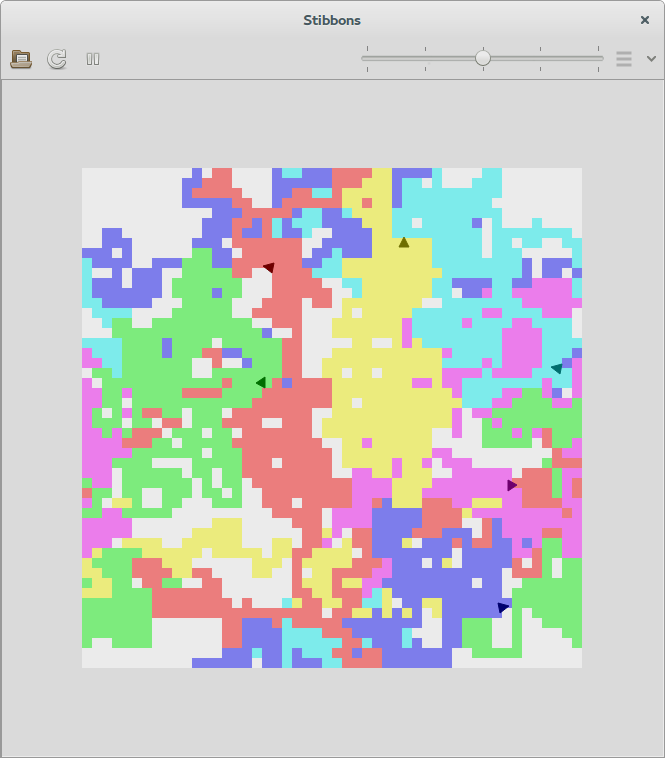
\includegraphics[scale=0.16]{doc/Presentation/screenshot/stibbons-0-4-2.png}
\end{center}

\begin{itemize}
	\item Plus de tortue par défaut
	\item Ouverture de plusieurs fichiers
	\item Démarrage, pause et redémarrage
	\item Gestion de la vitesse
	\item Export du modèle
	\item Bords rebouclants en option
\end{itemize}
\end{frame}

\begin{frame}
\frametitle{Application graphique v1.0}
\begin{center}
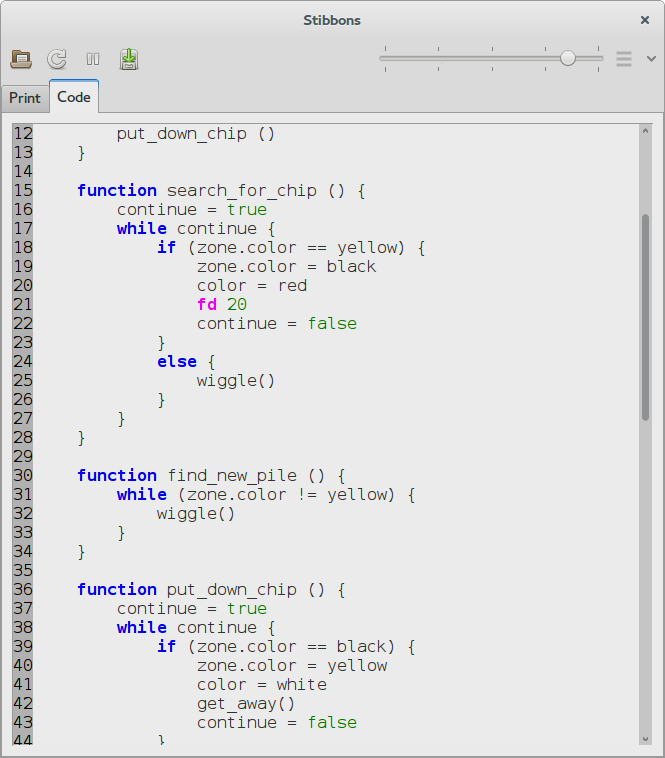
\includegraphics[scale=0.16]{doc/Presentation/screenshot/stibbons-0-5-2.png}
~~~~~~~~
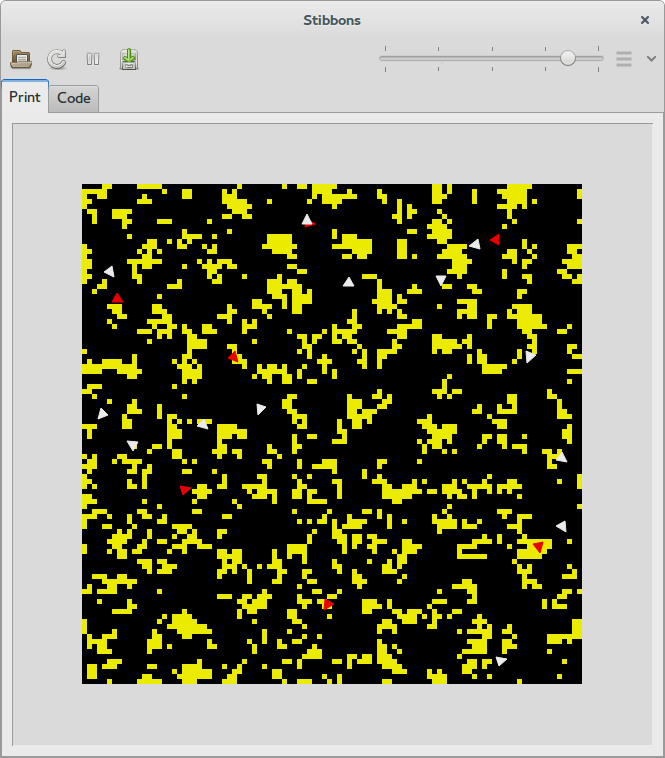
\includegraphics[scale=0.16]{doc/Presentation/screenshot/stibbons-0-5-3.png}
\end{center}

\begin{itemize}
	\item Editeur de programmes Stibbons
	\item Ajout de raccourcis clavier
	\item Bords rebondissants en option
\end{itemize}
\end{frame}

\begin{frame}
\frametitle{Application graphique v1.1}
\begin{center}
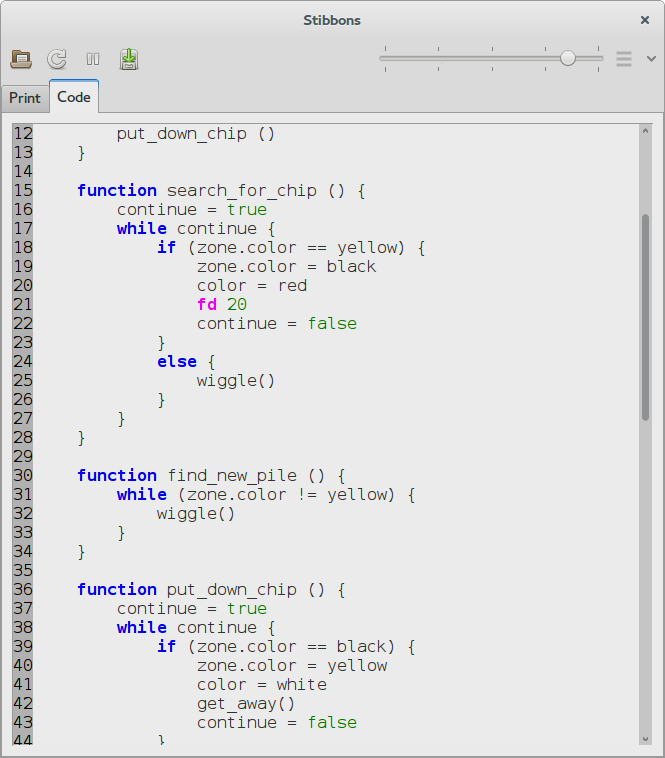
\includegraphics[scale=0.16]{doc/Presentation/screenshot/stibbons-0-5-2.png}
~~~~~~~~
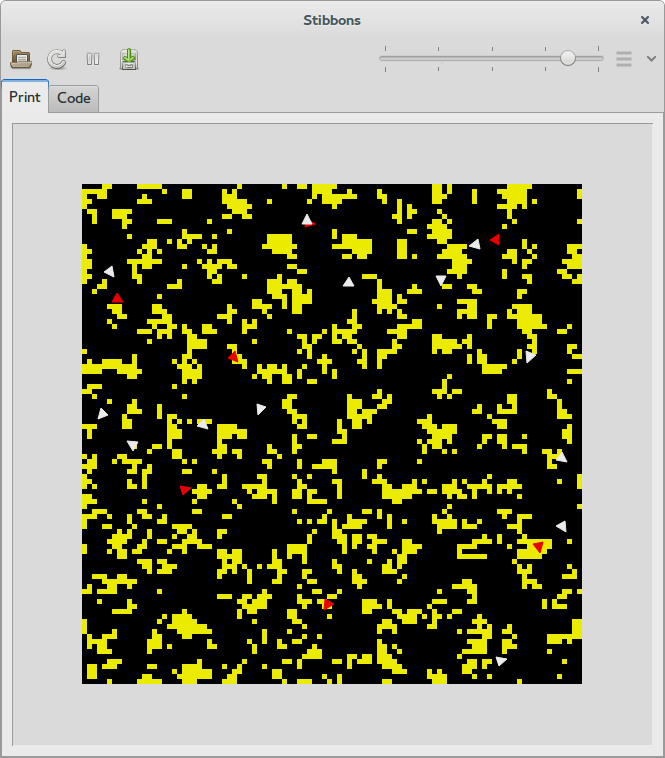
\includegraphics[scale=0.16]{doc/Presentation/screenshot/stibbons-0-5-3.png}
\end{center}

\begin{itemize}
	\item Correction d'une grave fuite mémoire
	\item Correction d'erreurs sémantiques
	\item Correction de la coloration syntaxique
\end{itemize}
\end{frame}

\subsection{Application CLI}

\begin{frame}[fragile]
\frametitle{Application CLI}
\begin{center}
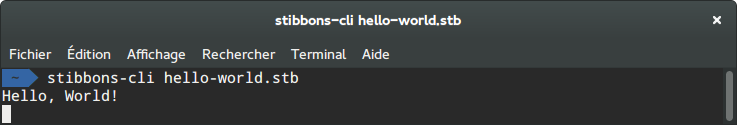
\includegraphics[scale=0.24]{doc/Presentation/screenshot/stibbons-cli.png}
\end{center}

\verb|stibbons-cli [options] fichier|

Options~:
\begin{description}
	\item[\texttt{-{}-}export s] Exporte le modèle toutes les \emph{s} secondes
	\item[\texttt{-{}-}prefix p] Préfixe les fichiers exportés avec \emph{p}
	\item[\texttt{-{}-}png] Génère une image PNG pour chaque export
	\item[\texttt{-{}-}no-json] N'exporte pas le modèle dans un fichier JSON
\end{description}

Arguments~:
\begin{description}
	\item[fichier] Le fichier de programme Stibbons à exécuter
\end{description}

\end{frame}



\section{Conclusion}
\begin{frame}
\begin{itemize}
\item Découverte de l'Agile
\item Diversité des outils
\item Améliorations à apporter à l'application
	\begin{itemize}
	\item formes des tortues
	\item largeur du pinceau
	\item parallélisme
	\item parcours d'arbre récursif $\rightarrow$ parcours à pile
	\item ...
	\end{itemize}
\end{itemize}
\end{frame}

\begin{frame}
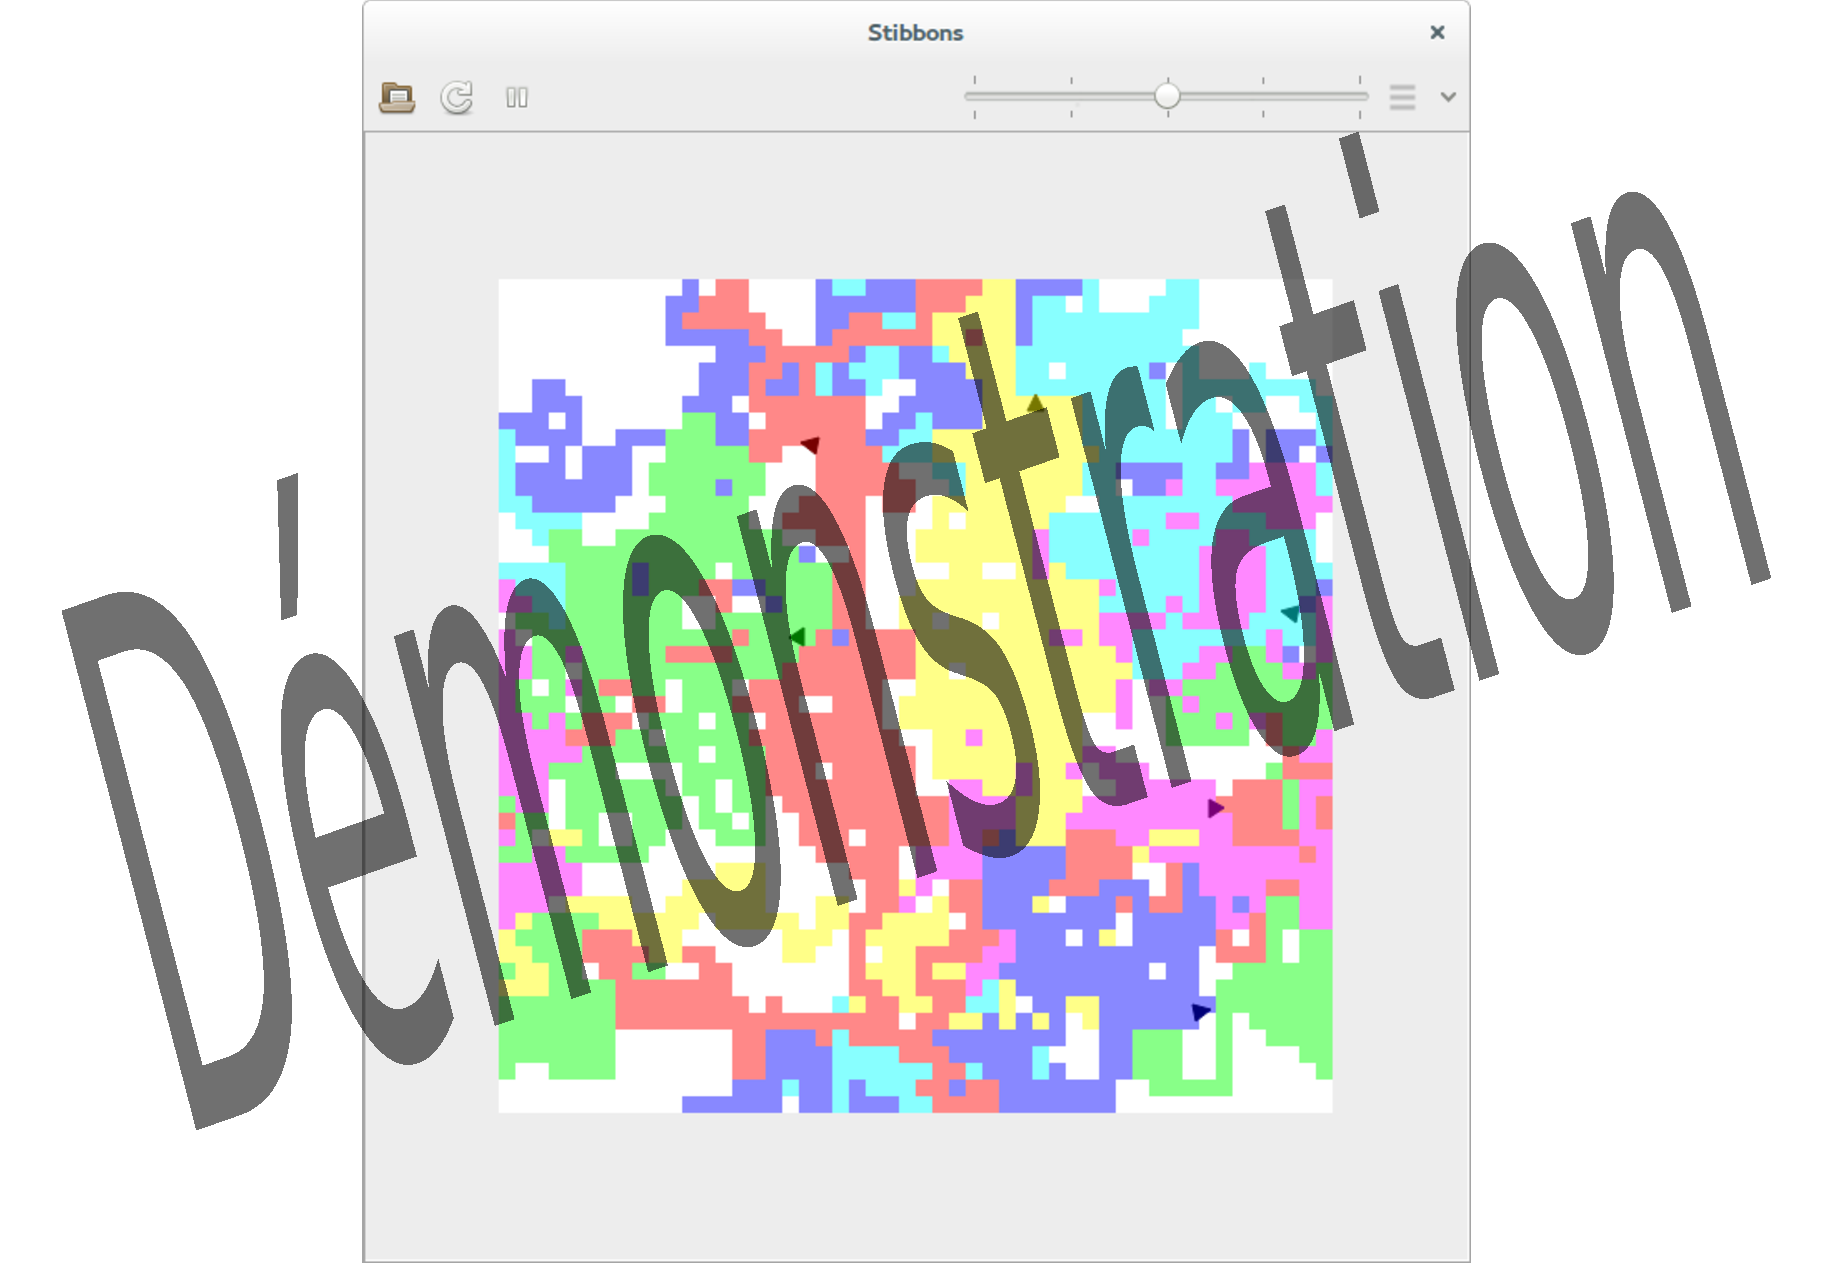
\includegraphics[scale=0.3]{doc/Presentation/image/demo.pdf}
\end{frame}


\end{document}


